\section{Introduction}

In this appendix, we demonstrate that \gls{lmrs} form sparse and large-diameter networks. Moreover, we provide exact bounds on the radius and the diameter of these networks based on their lattice type and the number of modules in the system.

We illustrate our demonstrations using the modular robots designed in the Smart Blocks and the Claytronics projects, namely the Smart Blocks, the millimeter-scale 2D Catoms, the Blinky Blocks and the 3D Catoms~\cite{piranda2016geom} (see Figure~\ref{fig:context:modular-robots}). These modular robots are arranged in the square, the hexagonal, the simple cubic, and the face-centered cubic lattices, respectively.

The analysis of the 3D-Catom system radius presented in this appendix was realized in cooperation with Thadeu Tucci, my office mate and PhD student.

The rest of this appendix is organized as follows. Section~\ref{section:appendixLMRs:related-work} presents the related work. Then, section~\ref{section:appendixLMRs:model} defines the system model and some terms. Afterwards, Section~\ref{section:appendixLMRs:density} characterizes the network density for our class of modular robots. Section~\ref{section:appendixLMRs:diameter} provides tight bounds of the radius and the diameter of the networks for our class of modular robots.

\section{Related Work}
\label{section:appendixLMRs:related-work}

To the best of our knowledge, little attraction has been paid to network characterization in the modular robotic community. In~\cite{garcia2009efficiency}, the authors compare the efficiency of neighbor-to-neighbor communication and global communication. Based on experimentally validated models, the authors compare the information transmission time in different scenarios for systems composed of 10 to 1000 modules. As mentioned in Section~\ref{section:context:classification}, global communication through a shared medium is less scalable with system size. Since we envision systems composed of millions of units, global communication is not an option.

As characterizing network properties is crucial for choosing appropriate algorithms and designing efficient new ones, graphs and networks have been extensively studied. Studies have been conducted on various graphs and networks, e.g., the Internet~\cite{latapy2006measuring,cardozoend,jin2006small}, the World Wide Web~\cite{albert1999internet}, sensor networks~\cite{jennings2002diameter}, small-world networks \cite{watts1998collective,hayes2000graph}, unit disk graphs~\cite{ellis2004random}, and lattice-based networks~\cite{hayes2000graph,barrenetxea2006lattice,barthelemy2011spatial}. These studies are network-specific. They are either measurement-based (e.g.,  \cite{latapy2006measuring,cardozoend,albert1999internet}), or purely theoretical using the intrinsic characteristics of the network (e.g., \cite{jennings2002diameter,ellis2004random,barrenetxea2006lattice,barthelemy2011spatial}).

Due to the regular tiling of the space in lattices, lattice-based networks obey certain geometric rules that can be used to analyze these networks. In~\cite{hayes2000graph, barrenetxea2006lattice}, the authors study some lattice-based networks, but they only consider networks embedded in the square lattice and restrict their analysis to specific network topologies, e.g., the square, the ring, etc. Their results are not generalizable to other lattices and arbitrary network topologies. In~\cite{barthelemy2011spatial}, the author states that the average distance between nodes in lattice networks is on the order of ${n}^{\frac{1}{D_L}}$, where $n$ is the number of nodes and $D_L$ is the dimension of the considered lattice.

In this appendix, we consider lattice-based networks embedded in any of the square, hexagonal, simple-cubic and face-centered lattices. We show that these networks are sparse and have a large diameter. Moreover, we provide tight lower and upper bounds for the radius and the diameter of these networks.

\section{System Model and Definitions}
\label{section:appendixLMRs:model}

In \gls{lmrs}, modules are arranged in some regular 2-dimensional or 3-dimensional lattice $L$. Here, we consider the Square (S), the Hexagonal (H), the Simple Cubic (SC) and the Face-Centered Cubic (FCC) lattices. Modules can only occupy a set of discrete positions defined by $L$. Note that modular robots may contain holes, i.e., some positions of $L$ may be unoccupied. As we assume neighbor-to-neighbor communications, $L$ also defines the module connectivity: Modules can directly communicate only with their immediate neighbors in $L$. $D_L$ denotes the dimension of $L$ and $\Delta_L$ represents its coordination number, i.e, the maximum number of modules to which a module can be connected.

Arbitrarily arranged modular robotic systems form lattice-based networks that can be modeled by connected, undirected, unweighted and lattice-based graphs $G = (V, E)$, where $V$ is the set of vertices (representing the modules), $E$ the set of edges (representing the connections), $|V|=n$, the number of vertices and $|E|= m$, the number of edges. $\delta(v_i)$ denotes $v_i$'s degree, i.e., the number of vertices to which $v_i$ is connected. $d(v_i,v_j)$ refers to the distance between the vertices $v_i$ and $v_j$, i.e., the number of edges on a shortest path between $v_i$ and $v_j$. The radius, $r$, and the diameter, $d$, of $G$ are respectively defined as $r = \min\limits_{v_i \in V}\ \max\limits_{v_j \in V}\ d(v_i,v_j)$ and $d = \max\limits_{v_i \in V}\ \max\limits_{v_j \in V}\  d(v_i,v_j)$. 

Notice that we assume a perfect alignment of the modules in the lattice. However, defects in the lattice, which may cause unreliable and intermittent connections, will only make the network sparser and increase both its radius and its diameter.

We now define some specific graphs used in this chapter. Let $V_L$ be the infinite set of vertices representing the infinite set of positions in $L$. The $\LSphere{L}(v_c,r)$ is a sphere embedded in $L$, where the vertex $v_c$ is the center of the sphere and $r \in \mathbb{N}$ its radius. It contains the set of vertices in $V_L$ whose distance from $v_c$ is equal to~$r$:

\begin{align}
\label{eq:def:sphere}
\LSphere{L}(v_c,r) = \{v_i \in V_L\ |\ d(v_i,v_c) = r\}
\end{align}

$\LBall{L}(v_c,r)$ is a ball embedded in $L$, where $v_c$ is the center of the ball and $r \in \mathbb{N}$ is its radius. It contains the set of vertices in $V_L$ whose distance from $v_c$ is less than or equal to~$r$:
\begin{align}
\label{eq:def:ball}
\LBall{L}(v_c,r) & = \{v_i\ \in V_L\ |\ d(v_i,v_c) \leq r\}\\
& = \bigcup\limits_{i=0}^{r} \LSphere{L}(v_c,i)
\end{align}

By an abuse of notation, $\LSphere{L}$ and $\LBall{L}$ can respectively refer to sphere and ball graphs embedded in $L$ where the connectivity between vertices is induced by the lattice structure of $L$. $\LSphere{L}(r)$ and $\LBall{L}(r)$ respectively refer to a sphere and a ball of radius $r$ in the lattice $L$. In all the illustrations of this chapter, $\LSphere{L}(r)$ is gradually colored from red to blue according to the value of $r$.

\newcommand{\assumptions}{Let $G = (V,E)$ be the network graph of an arbitrarily arranged modular robotic system that fits the model described in section~\ref{section:appendixLMRs:model}.\ }

\section{Network Density}
\label{section:appendixLMRs:density}

In this section, we show that the networks formed by our class of modular robots are all sparse.

\begin{cor}
	\label{corollaty:node-connectivity}
	\assumptions{} The vertex degree, $\delta(v_i)$, of any vertex $v_i \in V$ is bounded by:
	\begin{equation}
	0 \leq \delta(v_i) \leq \Delta_L
	\end{equation}
\end{cor}

\begin{lem}
	\label{edge-bounds}
	\assumptions{} The number of edges of $G$, $m$, is bounded as follows:
	\begin{align}
	n-1 \leq m \leq n\Delta_L 
	\end{align}
\end{lem}

\begin{pf}
	\textbf{Lower Bound.} A connected graph must have at least n-1 edges~\cite{hayes2000graph}.
	
	\noindent\textbf{Upper Bound.} Because of Corollary \ref{corollaty:node-connectivity}, every module cannot be connected to more than $\Delta_L$ others. Thus, the number of edges of $G$ is upper-bounded by $n\Delta_L$. Note that a tighter upper bound can be established by considering the lattice structure of $L$.
\end{pf}

\begin{thm}
	\assumptions{}  If $|V| = n$ is large, then $G$ is a sparse graph, i.e., $m \ll n^2$.	
\end{thm}

\begin{pf}
	If $n$ is large, then $\Delta_L \ll n$. Thus, we have $n \Delta_L \ll n^2$. Then, because of Lemma~\ref{edge-bounds},  we obtain $m \ll n^2$.
\end{pf}

\section{Network Radius and Diameter}
\label{section:appendixLMRs:diameter}

In this section, we establish tight lower and upper bounds of the radius and the diameter of the networks of our class of modular robots.

\subsection{Preliminary Materials}

This section presents some preliminary results used in the computations and the demonstrations of the radius and the diameter bounds of modular robot networks. We recall that $V_L$ is the infinite set of vertices representing the set of positions in the lattice $L$.

\begin{cor}
	\label{corollary:centrally-symmetric}
	$\forall v_c \in V_L,\ \forall r \in \mathbb{N},\  \LBall{L}(v_c,r)$ is centrally symmetric: The reflection $v_j$ of every vertex $v_i$ at distance $d(v_i,v_c) = k$ through $v_c$ is also at distance $k$ from $v_c$ and $d(v_i,v_j) = 2 k$.
\end{cor}

\begin{pf}	
	Let $\LBall{L}(v_c,1)$ be the ball of radius 1 and $v_c$ its center. All the vertices except $v_c$ are at distance 1 from $v_c$. Along every axis of the lattice $L$, two vertices, $v_1$ and $v_2$ are connected to $v_c$, one in each direction. These two vertices are symmetric through $v_c$, at distance 1 from $v_c$ and at distance 2 from each other.
	
	Let $\LBall{L}(v_c,r)$ be the ball of radius $r$ and $v_c$ its center. We assume that $\LBall{L}(v_c,r)$ is centrally symmetric. Let $\LBall{L}(v_c,r+1)$ be the ball of radius $r+1$ with $v_c$ being its center. By construction, $\LBall{L}(v_c,r+1)$ is obtained from $\LBall{L}(v_c,r)$ by adding all the vertices at distance $r+1$ from $v_c$. Let us consider $v_3$ and $v_4$ in $\LBall{L}(v_c,r)$ such that $v_3$ and $v_4$ are symmetric through $v_c$ and $d(v_3,v_4) = 2r$. In order to construct $\LBall{L}(v_c,r+1)$, we add to $v_3$ and $v_4$ two vertices $v_5$ and $v_6$ on the same axis but in the opposite direction such that $d(v_5,v_c) = d(v_6,v_c) = r+1$. $v_5$ and $v_6$ are symmetric through $v_c$. Moreover, there is no shortcut between $v_5$ and $v_6$, thus, $d(v_5,v_6) = 1 + d(v_3,v_4) + 1 = 2 + 2r = 2(r+1)$. Thus, $\LBall{L}(v_c,r+1)$ is centrally symmetric.
	
	By induction, $\forall v_c \in V_L,\ \forall r \in \mathbb{N},\ \LBall{L}(v_c,r)$ is centrally symmetric.
\end{pf}

\begin{lem}
	\label{lemma:radius-2diameter}
	$\forall v_c \in V_L,\ \forall r \in \mathbb{N}$, the diameter, $d$, of $\LBall{L}(v_c,r)$ is equal to $2r$.
\end{lem}

\begin{pf}
	As stated in Corollary~\ref{corollary:centrally-symmetric}, $\LBall{L}(v_c,r)$ is centrally symmetric. Thus, $\forall v_i \in \LBall{L}(v_c,r)$ such that $d(v_i, v_c) = r,\ \exists v_j \in \LBall{L}(v_c,r)$ with $d(v_i,v_j) = 2 r$. By construction, $\nexists v_i \in \LBall{L}(v_c,r),\ d(v_i,v_c) > r$. As a consequence, the diameter of $\LBall{L}(v_c,r)$, i.e., the largest distance between any two vertices, is equal to $d = 2 r$.
\end{pf}

\begin{cor}
	\label{corollary:radius-size}
	$\forall v_c \in V_L,\ \forall r \in \mathbb{N},\ \LBall{L}(v_c,r)$ is the minimum-radius and minimum-diameter existing graph composed of $n_{\LBall{L}}(v_c,r) = |\LBall{L}(v_c,r)|$ vertices in $L$.
\end{cor}

\begin{pf}
	By construction, in $\LBall{L}(v_c,r)$ all the positions of the lattice $L$ at a distance less than or equal to $r$ from $v_c$ are occupied. Thus, if we remove a vertex $v_1$ and add it to an empty place adjacent to a full one (the system should remain connected) occupied by the vertex $v_2$, the new location of $v_1$ must be at distance $r+1$ from $v_c$. Moreover, every vertex would be at distance $r+1$ or more from at least one other vertex. Thus, the radius of the graph would be equal to $r+1$.
	Moreover, because $\LBall{L}(v_c,r)$ is centrally symmetric (See Corollary~\ref{corollary:centrally-symmetric}), $\exists v_3 \in \LBall{L}(v_c,r),\ d(v_2,v_3) = 2 r$. Because of Lemma~\ref{lemma:radius-2diameter}, $d(v_2,v_3)$ is the diameter of $\LBall{L}(v_c,r)$. Since there is no shortcut between $v_1$ and $v_3$ in its new location, $d(v_1,v_3) =  d(v_2,v_3) + 1 = 2 r + 1$. Thus, the diameter of the graph would be equal to $2 r + 1$.
\end{pf}

\subsection{Radius and Diameter Bounds}

\begin{thm}
	\label{theorem:radius}
	\assumptions{} Let $\LBall{L}(r_b)$ and $\LBall{L}(r_b + 1)$ be two ball graphs embedded in $L$, such that the number of vertices of $G$, $n$, is between the number of vertices of these two balls, i.e.,  $n_{\LBall{L}}(r_b) \leq n < n_{\LBall{L}}(r_b+1)$. The radius, $r$, and the diameter, $d$, of $G$ are tightly bounded as follows:
	\begin{align} \label{eq:radius-diameter-bounds}
	r_b & \leq r \leq \lfloor \frac{n-1}{2} \rfloor\\
	2 r_b & \leq d \leq n-1
	\end{align}
\end{thm}

\begin{pf}
	\textbf{Upper Bound.} In a connected graph, any two vertices are at most separated by all the others. In such a graph, the $n$ vertices form a line of $n-1$ edges. Thus, the largest distance between any two vertices, i.e., the diameter of $G$, is at most equal to $n-1$ edges. The radius of $G$ is at most equal to the half of that line, i.e, $r \leq \lfloor \frac{n-1}{2} \rfloor$.\\
	\noindent\textbf{Lower Bound.} Because of Corollary~\ref{corollary:radius-size}, $\LBall{L}(r_b)$ is the minimum-radius and minimum-diameter graph composed of $n_{\LBall{L}}(r_b)$ vertices. Thus, with $n$ vertices, $G$ has a radius at least equal to $r_b$ and a diameter at least equal to the diameter of $\LBall{L}(r_b)$, which is, because of Lemma \ref{lemma:radius-2diameter}, equal to $2 r_b$.
\end{pf}

In the rest of this section, we establish the formula to compute the exact radius of an $\LBall{L}$ according to its number of vertices in the different lattices considered.

\paragraph{Systems in Two Dimensions: The Square and Hexagonal Lattices}

In this section, we compute the exact radius of an $\LBall{L}$, given the number of vertices it has, for the case of two-dimensional systems embedded in the Square (S) and Hexagonal (H) lattices. Figure~\ref{fig:appendixLMRs:s-h-ball} depicts an $\LBall{S}$ and an $\LBall{H}$ of radius 4, composed of Smart Blocks and 2D Catoms, respectively.

\begin{figure}[!h]
	\centering
	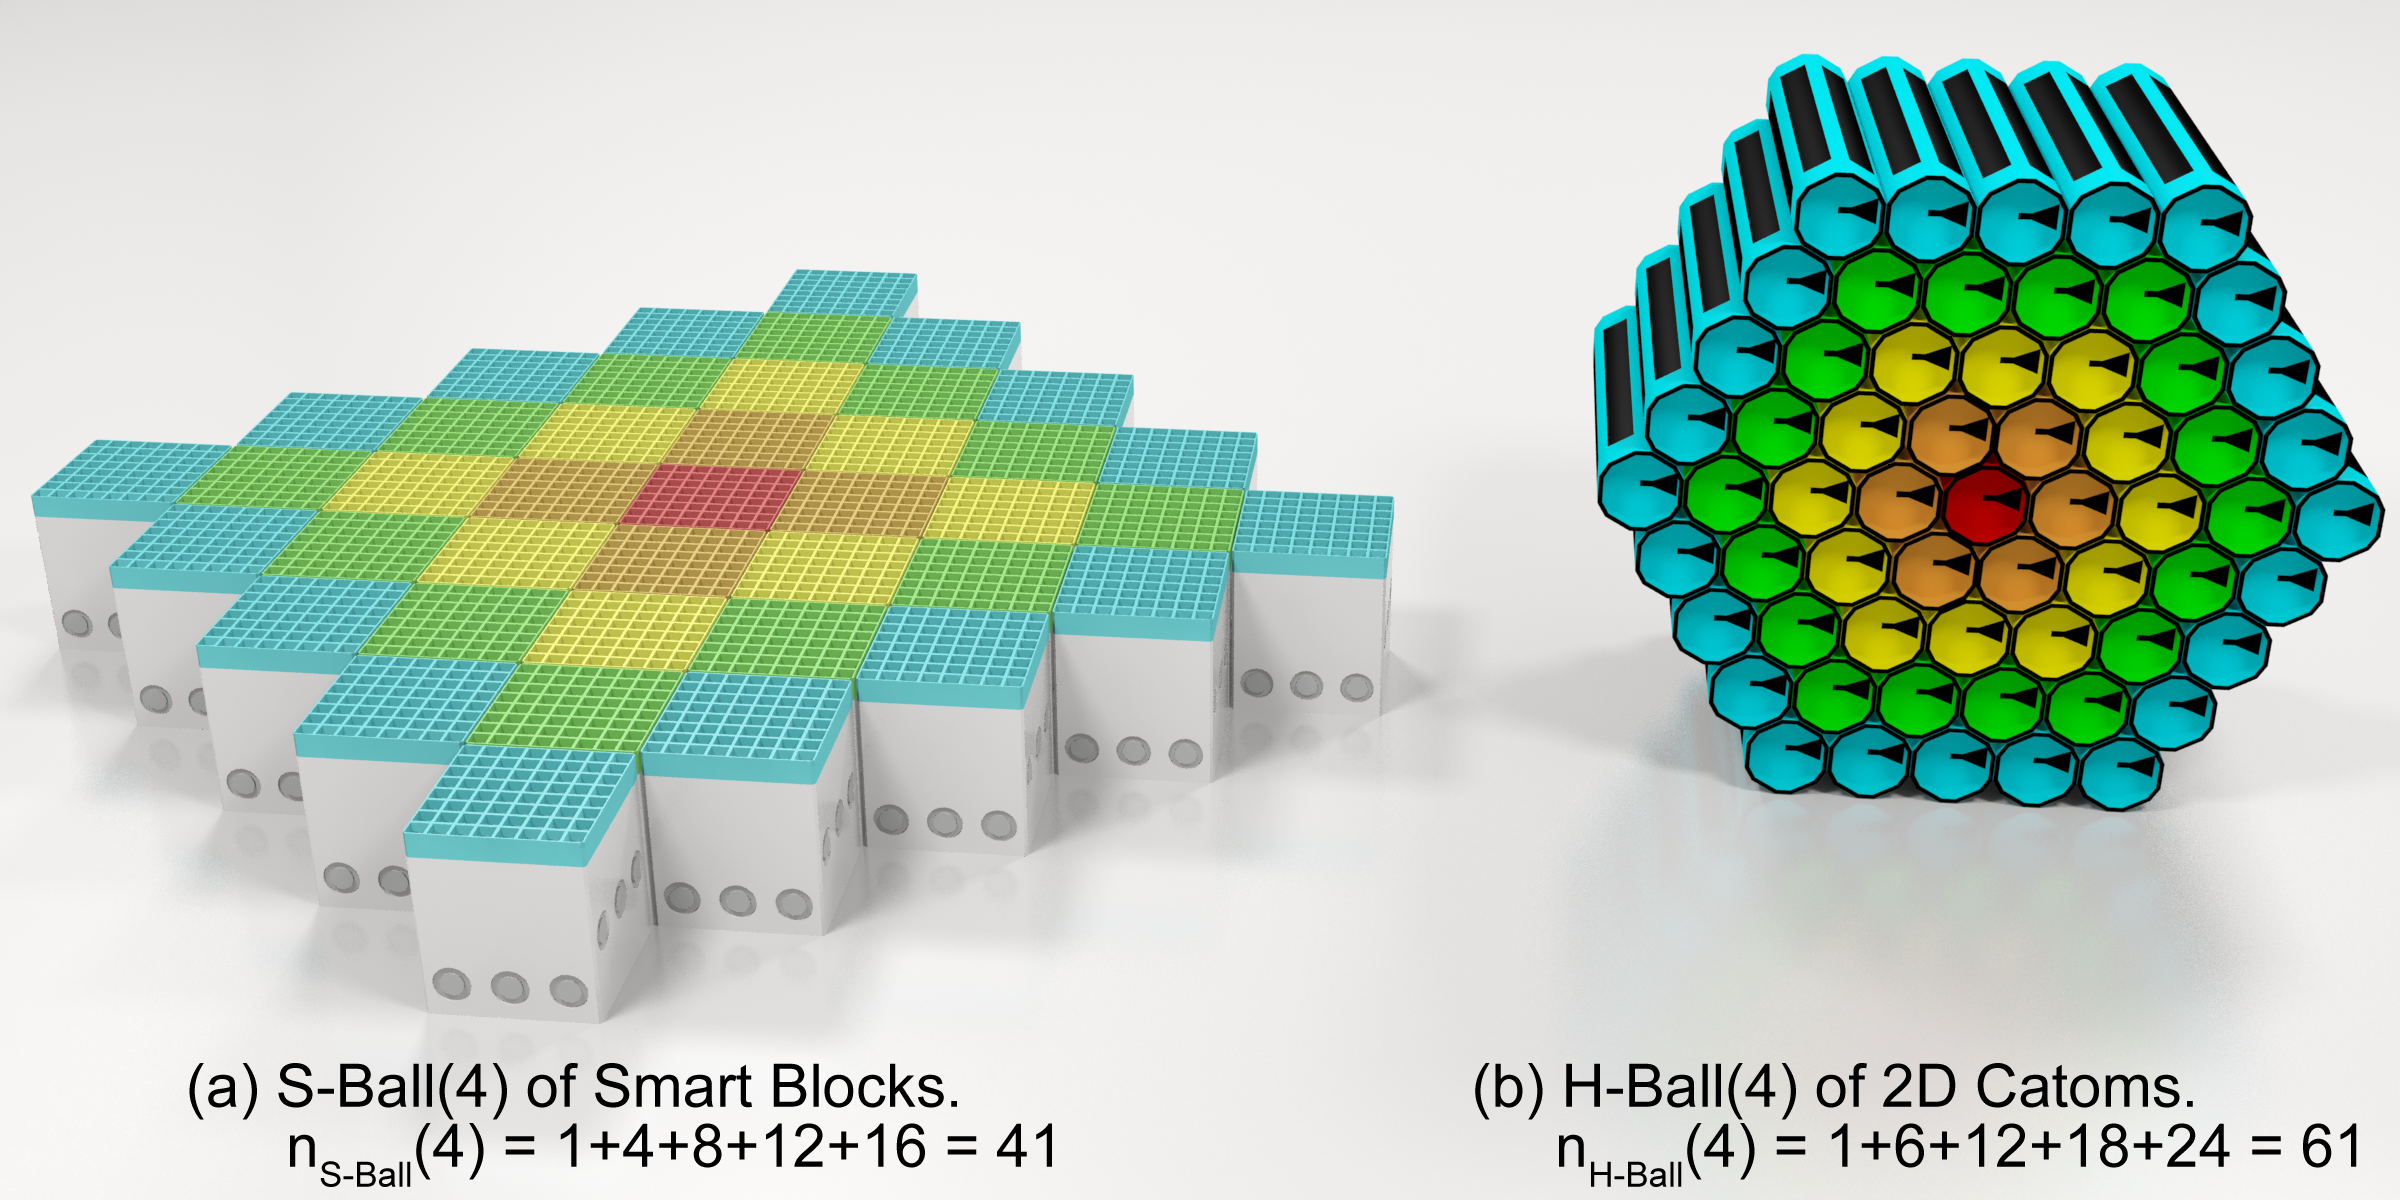
\includegraphics[width=0.65\linewidth]{images/network-characterization/ball-smartblocks-2dcatoms.png}
	\caption{An $\LBall{S}(4)$ and an $\LBall{H}(4)$ with color gradient from the center of the ball.\label{fig:appendixLMRs:s-h-ball}}
\end{figure}

\begin{lem}
	In the square and the hexagonal lattices, the number of vertices in a sphere of radius $r \geq 1$, $n_{\LSphere{L}}(r,\Delta_L)$, can be computed by:
	\begin{align}
	\label{eq:n-s-h-sphere}
	n_{\LSphere{L}}(r,\Delta_L) & =  r\Delta_L
	\end{align}
\end{lem}

\begin{pf}
	As illustrated in Figure~\ref{fig:appendixLMRs:s-h-ball}, in the square and the hexagonal lattices, a sphere of radius $r \geq 1$ is composed of $\Delta_L$ segments of length $r$ modules. Consequently, the number of vertices is equal to $r \Delta_L$.
\end{pf}

\begin{thm}
	In the square and the hexagonal lattices, the radius of a ball composed of $n \geq 1$ vertices, $r_{\LBall{L}}(n,\Delta_L)$, can be computed by:
	\begin{align}
	\label{eqn:radius-2d}
	r_{\LBall{L}}(n,\Delta_L) & = \frac{1}{2} \left( \sqrt{1+\frac{8(n-1)}{\Delta_L}} - 1 \right)
	\end{align}
\end{thm}

\begin{pf}
	By definition, $\LBall{L}(r)$ is the union of all the $\LSphere{L}(i)$ for $i$ ranging from $0$ to $r$. Thus, in the square and the hexagonal lattices, for $r \geq 1$, the number of vertices in an $\LBall{L}(r)$, $n_{\LBall{L}}(r,\Delta_L)$, can be computed as follows:
	\begin{align}
	n_{\LBall{L}}(r,\Delta_L) & = \sum_{i=0}^{r} n_{\LSphere{L}}(i, \Delta_L) \\
	& =  1 + \sum_{i=1}^{r} i \Delta_L \\ 
	& = \frac{1}{2} {r}^2 \Delta_L + \frac{1}{2} r \Delta_L + 1
	\label{eq:n-s-h-ball}
	\end{align}
	To obtain Equation~\ref{eqn:radius-2d}, we solve Equation \eqref{eq:n-s-h-ball} for $r$ and keep only the positive root.
\end{pf}

\paragraph{Systems in Three Dimensions: The Simple Cubic and Face-Centered Cubic Lattices}

In this section, we compute the exact radius of an $\LBall{L}$, given the number of vertices it contains, for the case of three-dimensional systems embedded in the Simple Cubic (SC) and Face-Centered Cubic (FCC) lattices. Figures~\ref{fig:appendixLMRs:sc-ball} and \ref{fig:appendixLMRs:fcc-ball} depict the $\LBall{SC}$ and the $\LBall{FCC}$ of radius 2, composed of Blinky Blocks and 3D Catoms, respectively. Both systems can be decomposed into horizontal layers.

\subparagraph{\textbf{The Simple Cubic Lattice}}
\label{section:appendixLMRs:diameter-blinkyblocks}

\begin{figure}[!h]
	\centering
	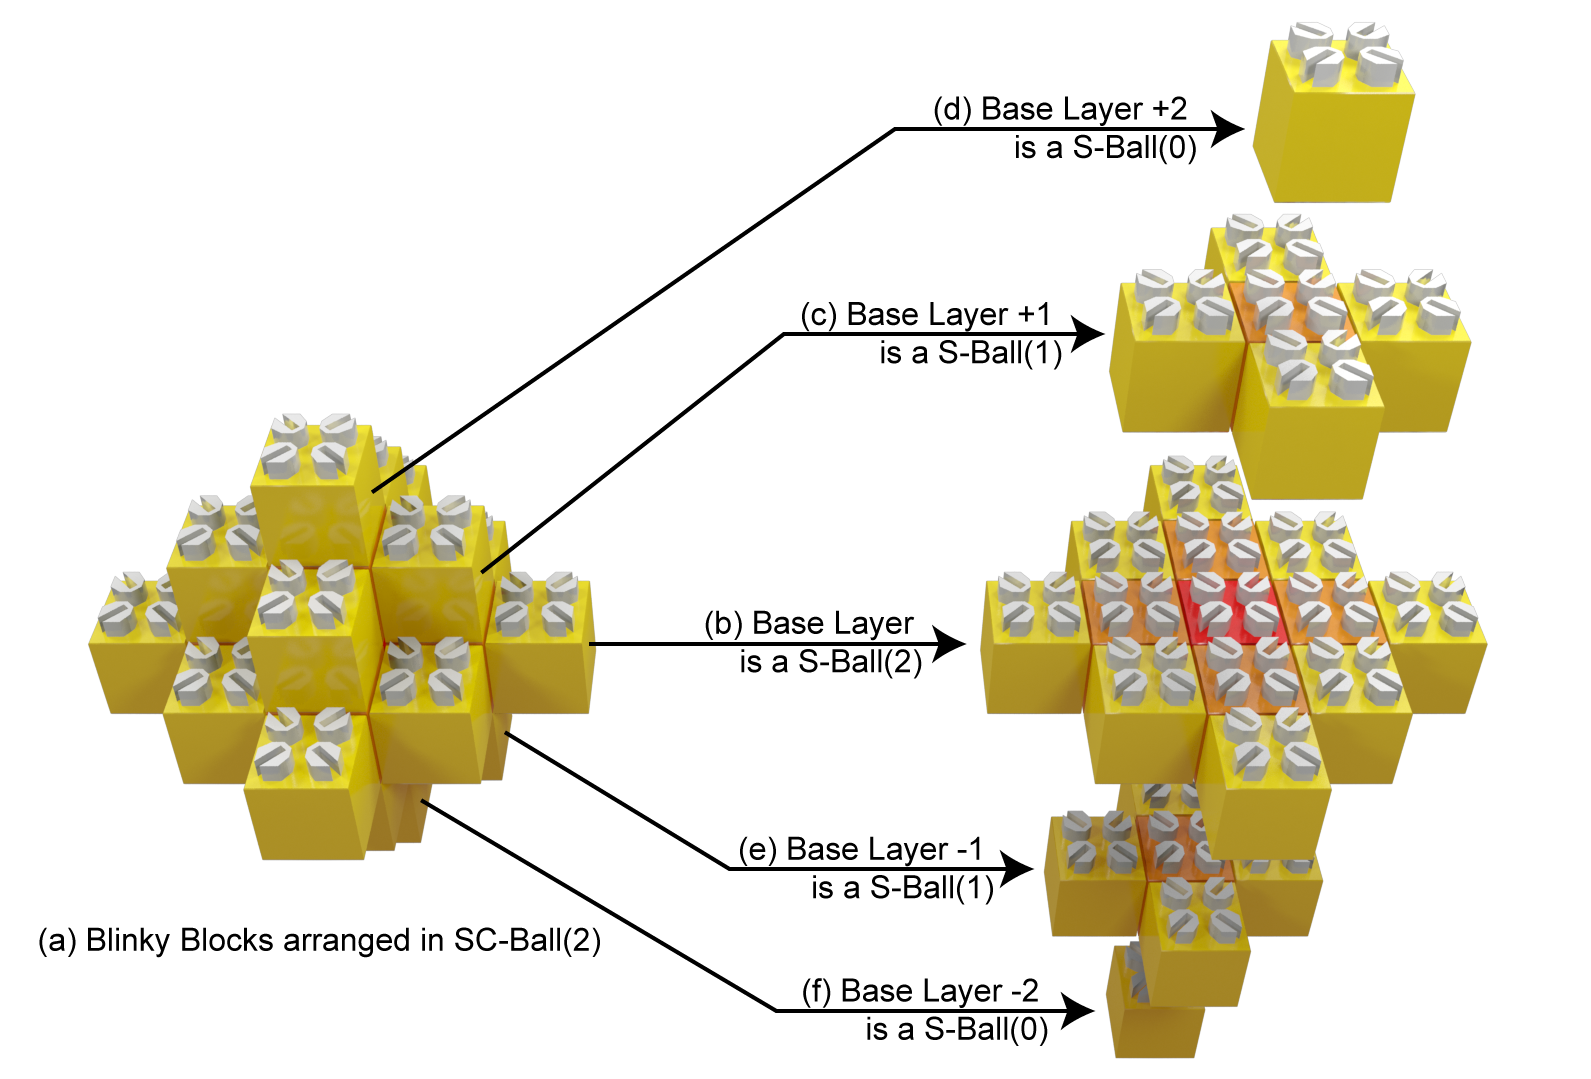
\includegraphics[width=0.8\linewidth]{images/network-characterization/ball-blinkyblocks.png}
	\caption{An $\LBall{SC}(2)$ of Blinky Blocks and its decomposition into horizontal layers with color gradient from the center of the ball.\label{fig:appendixLMRs:sc-ball}}
\end{figure}

\begin{lem}
	In the simple cubic lattice, the number of vertices in a sphere of radius $r \geq 1$, $n_{\LSphere{SC}}(r)$, can be computed by:
	\begin{align}
	\label{eq:n-sc-sum-sphere}
	n_{\LSphere{SC}}(r) & = n_{\LSphere{S}}(r) + 2\sum_{i=0}^{r-1} n_{\LSphere{S}}(i)\\
	& = 2 (2r^2 + 1)
	\label{eq:n-sc-sphere}
	\end{align}
\end{lem}

\begin{pf}
	As illustrated in Figure~\ref{fig:appendixLMRs:sc-ball}, a sphere of radius $r$ in the simple cubic lattice can be decomposed into  $2r + 1$ horizontal $\LSphere{S}s$ of different radii. Equation~\eqref{eq:n-sc-sum-sphere} is obtained by summing up all the sizes of the $\LSphere{S}s$.
\end{pf}

\begin{thm}
	In the simple-cubic lattice, the radius of a ball composed of $n \geq 1$ vertices, $r_{\LBall{SC}}(n)$, can be computed by: 
	\begin{equation}
	\label{eqn:radius-3d-sc}
	r_{\LBall{SC}}(n) = \frac{1}{2} \left(\frac{(\sqrt{3} \sqrt{243 n^2+125}+27 n)^\frac{1}{3}}{3^{\frac{2}{3}}}-\frac{5}{3^{\frac{1}{3}} (\sqrt{3} \sqrt{243 n^2+125}+27 n)^{\frac{1}{3}}} - 1\right)
	\end{equation}
\end{thm}

\begin{pf}
	By definition, $\LBall{L}(r)$ is the union of all the $\LSphere{L}(i)$ for $i$ ranging from $0$ to $r$. Thus, for $r \geq 1$, the number of vertices in an $\LBall{SC}(r)$, $n_{\LBall{SC}}(r)$, can be computed as follows:
	\begin{align}
	n_{\LBall{SC}}(r) & = \sum_{i=0}^{r} n_{\LSphere{SC}}(i) \\
	& =  1 + \sum_{i=1}^{r} 2 (2i^2 + 1)\\
	& = \frac{4}{3} r^3 + 2 r^2 + \frac{8}{3}r + 1
	\label{eq:n-sc-ball}
	\end{align}
	To obtain Equation~\ref{eqn:radius-3d-sc}, we solve Equation~\eqref{eq:n-sc-ball} for $r$ and keep only the real root.
\end{pf}

\subparagraph{\textbf{The Face-Centered Cubic Lattice}}

\begin{figure}[!h]
	\centering
	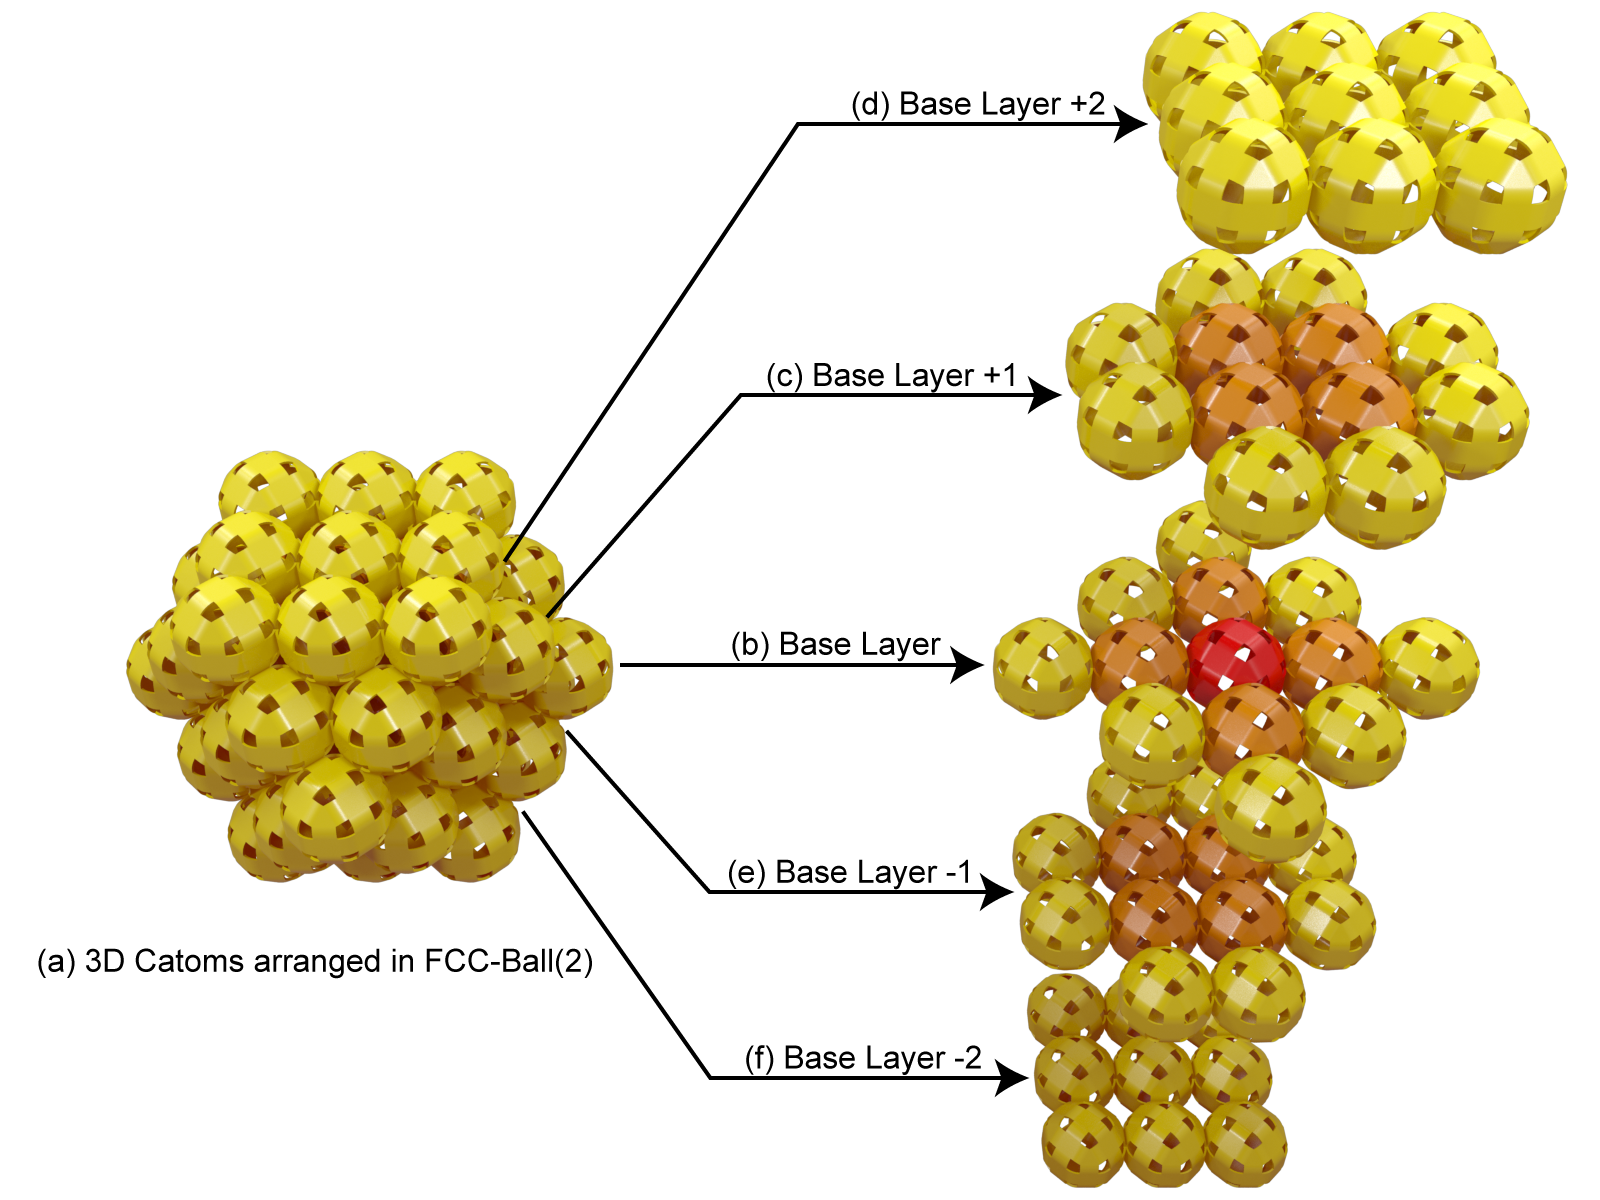
\includegraphics[width=0.8\linewidth]{images/network-characterization/ball-3dcatoms.png}
	\caption{An $\LBall{FCC}(2)$ of 3D Catoms and its decomposition into horizontal layers with color gradient from the center of the ball.\label{fig:appendixLMRs:fcc-ball}}
\end{figure}

\begin{lem}
	In the face-centered cubic lattice, the number of vertices in a sphere of radius $r \geq 1$, $n_{\LSphere{FCC}}(r)$, can be computed by:
	\begin{align}
	\label{eq:n-fcc-sum-sphere}
	n_{\LSphere{FCC}}(r) &  = 4r + 2(r+1)^2 + 2(r-1)4r\\
	\label{eq:n-fcc-sphere}
	& = 2 (5r^2 + 1)
	\end{align}
\end{lem}
\begin{pf}
	As shown in Figure~\ref{fig:appendixLMRs:fcc-ball}, a sphere of radius $r$ in the face-centered cubic lattice can be decomposed into $2r + 1$ horizontal layers. The base layer is an $\LSphere{S}(r)$ and contains $4r$ vertices. The bottom and the top layers both contain $(r+1)^2$ vertices. The $2(r-1)$ other layers contain $4r$ vertices each. Equation~\eqref{eq:n-fcc-sum-sphere} is obtained by summing up the number or vertices of each layer.
\end{pf}

\begin{thm}
	In the face-centered cubic lattice, the radius of a ball of $n \geq 1$ vertices, $r_{\LBall{FCC}}(n)$, can be computed by:
	\begin{multline}
	\label{eqn:radius-3d-fcc}
	r_{\LBall{FCC}}(n) = \frac{1}{2} \left(\frac{(\sqrt{15} \sqrt{4860 n^2+343}+270 n)^\frac{1}{3}}{15^{\frac{2}{3}}} - 	\frac{7}{15^{\frac{1}{3}} (\sqrt{15} \sqrt{4860 n^2+343}+270 n)^{\frac{1}{3}}} - 1\right)
	\end{multline}
\end{thm}

\begin{pf}
	By definition, $\LBall{L}(r)$ is the union of all the $\LSphere{L}(i)$ for $i$ ranging from $0$ to $r$. Thus, for $r \geq 1$, the number of vertices in an $\LBall{FCC}(r)$, $n_{\LBall{FCC}}(r)$, can be computed as follows:
	\begin{align}
	n_{\LBall{FCC}}(r) & = \sum_{i=0}^{r} n_{\LSphere{FCC}}(i) \\
	& =  1 + \sum_{i=1}^{r} 2 (5i^2 + 1)\\
	& = \frac{10}{3} r^3 + 5r^2 + \frac{11}{3}r + 1
	\label{eq:n-fcc-ball}
	\end{align}
	To obtain Equation~\ref{eqn:radius-3d-fcc}, we solve Equation~\eqref{eq:n-fcc-ball} for $r$ and keep only the real root.
\end{pf}
